\begin{figure}
	\centering
	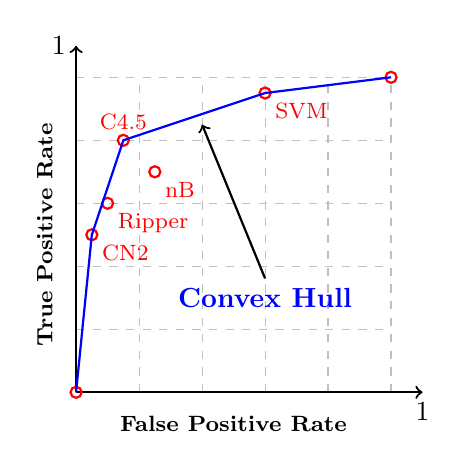
\begin{tikzpicture}[
		scale=4.0
	]

		\draw[step=0.2,lightgray,dashed] (0,0) grid (1,1);

		% axes
		\draw[->,thick] (0,0) -- (1.1,0) node[below]{1};
		\draw[->,thick] (0,0) -- (0,1.1) node[left]{1};

		\node at (0.5,-0.1) {\footnotesize\textbf{False Positive Rate}};
		\node[rotate=90] at (-0.1,0.5) {\footnotesize\textbf{True Positive Rate}};

		\draw[red,thick] (0,0) circle (0.5pt);
		\draw[red,thick] (0.05,0.5) circle (0.5pt) node[below right]{\footnotesize CN2};
		\draw[red,thick] (0.1,0.6) circle (0.5pt) node[below right]{\footnotesize Ripper};
		\draw[red,thick] (0.25,0.7) circle (0.5pt) node[below right]{\footnotesize nB};
		\draw[red,thick] (0.15,0.8) circle (0.5pt) node[above]{\footnotesize C4.5};
		\draw[red,thick] (0.6,0.95) circle (0.5pt) node[below right]{\footnotesize SVM};
		\draw[red,thick] (1,1) circle (0.5pt);

		\draw[blue,thick] (0,0) -- (0.05,0.5) -- (0.15,0.8) -- (0.6,0.95) -- (1,1);

		\node[blue] (A) at (0.6,0.3) {\textbf{Convex Hull}};
		\draw[->,thick] (A.north) -- (0.4,0.85);
		
	\end{tikzpicture}
\end{figure}